\chapter{Deciding that a service is behaving abnormally}
\label{ch:detect}

\section{The core idea: normal is personal}
\begin{simplebox}
What is a normal number? It depends on who you ask. A database might use 40\% of its memory all day, and that is normal for it. A tiny helper service might use 2\%. A rule such as ``alarm if memory is over 80\%'' is wrong for both of them. So instead of one rule for everyone, we compare every service with \emph{its own recent past}. If the database suddenly uses 90\% when it usually uses 40\%, that is unusual \emph{for the database}.
\end{simplebox}

\begin{techbox}
Services differ by orders of magnitude in every metric, so global thresholds fail. Each service is judged against its own recent window of readings, using robust statistics: the median for location and the median absolute deviation (MAD) for spread, because a mean and standard deviation are dragged by the very outliers we are trying to detect. A robust $z$ is $(x-\operatorname{median})/(1.4826\cdot\mathrm{MAD})$, and the constant 1.4826 makes MAD comparable to a standard deviation for Gaussian data.
\end{techbox}

\section{Engine 1: the rules}
\begin{simplebox}
The rule engine is the simple one. For each of the eight numbers it asks ``how many robust standard deviations away from this service's normal is it right now?'' and only cares about the bad direction (CPU going up, not down). If that distance passes a line (three), the service is flagged. Container facts (stopped, paused, crash-looping) are also flagged outright.

Strengths: very easy to explain, reacts fast to loud faults. Weaknesses: it fires on ordinary noise, so it raises the most false alarms, and it blames the loudest service, which is often a victim.
\end{simplebox}

\begin{techbox}
A robust one-sided $z$-score per metric (median and MAD, bad direction only) gives a rule score $\rho_s$ normalised so that $1$ is its three-sigma line. Settings include \code{minHistorySamples}=12, \code{zScoreAnomaly}=3.5, \code{zScoreHigh}=5, \code{zScoreCritical}=8, \code{minDeltaPercent}=5 (a large $z$ is ignored unless the metric moved at least 5 percentage points, so an idle service going from 0.05\% to 2\% CPU does not raise an incident), and absolute thresholds of 70\% (high) and 85\% (critical) for CPU and memory. Measured on the 62 real faults the rules detect 90\%, catch-and-name 63\%, raise 9.2 false-alarm episodes per fault-free hour and spend 9\% of the time in alarm.
\end{techbox}

\section{Engine 2: the old ML, an Isolation Forest per service}
\begin{simplebox}
An Isolation Forest is a way to find ``odd one out'' points. Imagine a pile of marbles on a table. If you draw random lines through the pile, a marble sitting far from the pile gets separated from the rest after only a few lines, while a marble in the middle takes many cuts. The fewer cuts it takes to isolate a point, the more unusual it is.

We trained two of these per service on its recent readings. They are good at ``this reading is unlike the recent ones''. And that is exactly their weakness: when the \emph{whole system} gets quieter, every service's readings are unlike the recent ones, so everything looks odd at once.
\end{simplebox}

\begin{techbox}
Isolation Forest (Liu, Ting and Zhou, 2008) isolates an outlier with few random cuts, with the anomaly score a monotone function of the expected path length. It needs no density estimate, which suits mixed, skewed metrics. The first engine used two forests per service (one over ``own'' resource signals, one over ``symptom'' signals), plus a range guard, and a 30-minute wait before accepting a large shift as the new normal. A forest cannot score a value beyond its training range higher than its most extreme training point, so the engine added a range guard; but that guard fires for every service when traffic changes for all of them.
\end{techbox}

\section{Engine 3: the new ML, the load-aware residual model}
\label{sec:loadmodel}
This is the part to understand best, because it is the contribution that came out of the failure.

\subsection{Step 0: the picture}
\begin{simplebox}
Imagine ten shops on one street. On a rainy day, every shop gets fewer customers. If you check each shop separately against its own history, every shop looks ``abnormally quiet'' and you think ten shops are broken. A smarter check first asks: \emph{how quiet is the whole street?} If the street is down by half, you expect every shop to be down by about half. Then you look for the shop that is down by \emph{more} than half, or the one that is up when the others are down. \emph{That} shop has a real problem.

This is the entire idea. Estimate the shared change, expect each service to follow it, and look at the leftover.
\end{simplebox}

\subsection{Step 1: put numbers on a log scale}
\begin{simplebox}
Traffic changes are multiplicative: ``twice as busy'' matters whether the service handled ten requests or ten thousand. A log scale turns ``twice as much'' into the same step everywhere. We also add a small ``unit'' so that tiny flickers on an idle service (a 1\% CPU blip) do not look like big events.
\end{simplebox}

\begin{techbox}
Each signal is $x_{s,f}=\log(v_{s,f}+u_f)$ with units $u_f=5$ for CPU (so a one-point blip on an idle service is no event), $1$ for memory, $2000$\,B/s for network and $0.1$ for request rate. A missing signal stays missing.
\end{techbox}

\subsection{Step 2: a slow reference}
\begin{simplebox}
For each number of each service we keep a ``reference'': the typical value over the last half hour. We take the \emph{median} (the middle value), not the average, so one weird spike does not move it. Everything is then measured as ``how far above or below its own reference is it right now?''
\end{simplebox}

\begin{techbox}
$r_{s,f}$ is the median of the service's last $360$ readings (half an hour at 5\,s). A short quiet spell does not move it. The shift is $d_{s,f}(t)=x_{s,f}(t)-r_{s,f}$.
\end{techbox}

\subsection{Step 3: measure the shared change (the load factor)}
\begin{simplebox}
Now take all the services that carry traffic and ask: on average, how far have they all moved right now? Use the \emph{median} of their moves. A median is the middle one when you line them up. If one service goes crazy, it is only one number at the end of the line, and the middle barely moves. If \emph{every} service moves up, the middle moves up. That is exactly the behaviour we want: the load factor follows the shared change and ignores a single broken service.

An idle database that always reads zero says nothing about traffic, so we only use signals that actually carry traffic (their reference is clearly above idle).
\end{simplebox}

\begin{techbox}
A signal \emph{carries traffic} if $r_{s,f}-\log u_f\ge 0.4$. Over the carrying signals of network in/out, request rate and CPU, the load factor is
\[
L(t)=\operatorname*{median}_{(s,f)\in\mathcal A(t)}\ d_{s,f}(t),
\]
taken only when at least two services contribute. $e^{L}$ is the factor by which the project's traffic changed; the Detection engines page shows it as a chip (``workload steady'' or ``traffic $\times$2.4, explained, not a fault'').
\end{techbox}

\begin{examplebox}[Worked example: ten services, one broken]
Nine busy services each move by about $+0.7$ on the log scale (traffic roughly doubled; $e^{0.7}\approx2$). One service, \code{payment}, moves by $+3.0$ because it is also in trouble. Sort the ten moves: $0.6,0.65,0.7,0.7,0.7,0.7,0.75,0.8,0.85,3.0$. The median is the average of the 5th and 6th, $(0.7+0.7)/2=0.7$. The load factor is $0.7$, not dragged by \code{payment}'s $3.0$. Expected move for each service is about $0.7$. \code{payment}'s leftover is $3.0-0.7=2.3$, which is large; the others' leftovers are about $0.0$ to $0.15$. Only \code{payment} stands out.
\end{examplebox}

\subsection{Step 4: some signals follow the load, some ignore it}
\begin{simplebox}
Not everything follows traffic. A gateway's network use goes up with traffic. A message bus idling in the corner may stay the same. The mapper learns, for each kind of signal, how strongly it follows the shared change in \emph{this} project, by comparing the past shared change with the past movement of those signals. If it has not seen enough load changes to learn, it uses a sensible starting guess (network and requests follow load about one-for-one, CPU about 0.4).
\end{simplebox}

\begin{techbox}
The slope $b_f$ is a ridge regression of the shifts $d_{s,f}(\tau)$ on $L(\tau)$ over the carrying signals in the stored window:
\[
b_f=\frac{\sum d\,L+\kappa\,b^0_f}{\sum L^2+\kappa},\qquad \kappa=60,
\]
with priors $b^0=1$ for network and requests and $0.4$ for CPU. The ridge term pulls the slope towards the prior until the data say otherwise.
\end{techbox}

\subsection{Step 5: judge the leftover, under two excuses}
\begin{simplebox}
Here is the clever safety trick. For each number we try two excuses. Excuse one: ``this signal ignores the load'' (so expect no change). Excuse two: ``this signal follows the load'' (so expect it to have moved with the street). If \emph{either} excuse explains the reading, it is not unusual. A reading is flagged only if \emph{neither} excuse can explain it. This keeps us from raising false alarms while the load changes, and keeps us from missing a real fault that happens during a load change: a CPU spike on one service during a traffic surge is still a spike compared with what the surge predicts.
\end{simplebox}

\begin{techbox}
For each hypothesis $b\in\{0,b_f\}$, the window of the service's \emph{accepted} readings gives a baseline $m^{(b)}$ (the median of $x_{s,f}(\tau)-bL(\tau)$) and a robust spread $\sigma^{(b)}$. The deviation is
\[
z_{s,f}=\min_{b\in\{0,\,b_f\}}\ \frac{\lvert x_{s,f}-bL-m^{(b)}\rvert}{\sigma^{(b)}},
\]
so a signal counts as unusual only if neither way of following the load explains it. Only \emph{increases} of CPU, memory, throttling, errors and latency count (less of them never signals a fault of the service itself and follows every restart); traffic counts in both directions. The service's level is $\max_f z_{s,f}/z_{\text{line}}$ with $z_{\text{line}}=4$, so level $1$ is the service's own alarm line and the hybrid uses level $2$ ($z=8$). The strongest signal and its $z$ are kept, so the verdict reads ``CPU 9.3 spreads from what the load predicts''.
\end{techbox}

\subsection{Step 6: how wide is ``normal''? The tail-aware spread}
\begin{simplebox}
Some numbers are \emph{bursty}: they are quiet most of the time and jump every few minutes even when nothing is wrong (think batch jobs). If you measure the spread of such a number in the usual way, the spread looks tiny, so an ordinary burst looks like a five-alarm event. We fix this by making the spread at least as wide as the distance from the typical value to the 90th-percentile value, in the direction we care about. A burst that happens regularly is then part of the normal width.
\end{simplebox}

\begin{techbox}
$\sigma=\max\bigl(1.4826\,\mathrm{MAD},\ (q_{0.90}-m)/1.2816,\ \phi_f\bigr)$ for the upper tail, or both tails for two-sided signals, with a floor $\phi_f$ at the smallest change worth noticing (floors $[0.2,0.05,0.3,0.3,0.3,0.02,0.2,3]$ over the eight signals). The MAD alone treats a bursty signal as Gaussian and alarms on its ordinary bursts. Measured effect: with the MAD spread instead of the tail-aware one, alarm time on the workload recordings rises from 0\% to 10\% and 6\%, and on the real systems it doubles from 6\% to 12\%.
\end{techbox}

\subsection{Step 7: do not learn from your own alarms}
\begin{simplebox}
The model learns what normal looks like from recent readings, but with a rule: \emph{only readings that were not alarming are allowed into the learning window.} Otherwise a long fault would slowly teach the model that the fault is normal, and the alarm would fade. There is one exception, on purpose. If a service settles at a new level that is only slightly unusual, and stays there for two minutes, we accept it as the new normal. A big shift is only accepted after thirty minutes. This way a service that really did change (after a deploy, say) stops alarming forever, but a real fault does not get absorbed quickly.
\end{simplebox}

\begin{techbox}
Only readings under level $1$ join the window of $W=120$ readings. A small steady shift (level below $3$) is accepted as the new normal after $24$ readings (two minutes), a large one after $360$ (thirty minutes). A service is judged only after $30$ readings. Baselines are cached and refreshed every four readings. The price: a mild fault that lasts longer than two minutes is eventually absorbed and the model stops alarming on it, while the rule layer and the container facts of the hybrid keep alarming. Raising the two-minute setting to 4--20 minutes changed nothing on accuracy but doubled alarm time on the real systems from 6\% to 13\%, so we kept two minutes.
\end{techbox}

\begin{warnbox}
This absorbed-fault behaviour is a real limitation, and you will see it in the live demo of the simulator: the ML engine alarms on the slow \code{payment} fault for about 48 simulated seconds, then goes quiet, while the Rules and Hybrid keep alarming. Say so before an evaluator notices it.
\end{warnbox}

\subsection{Summary of the model in one picture}
\begin{figure}[H]
\centering
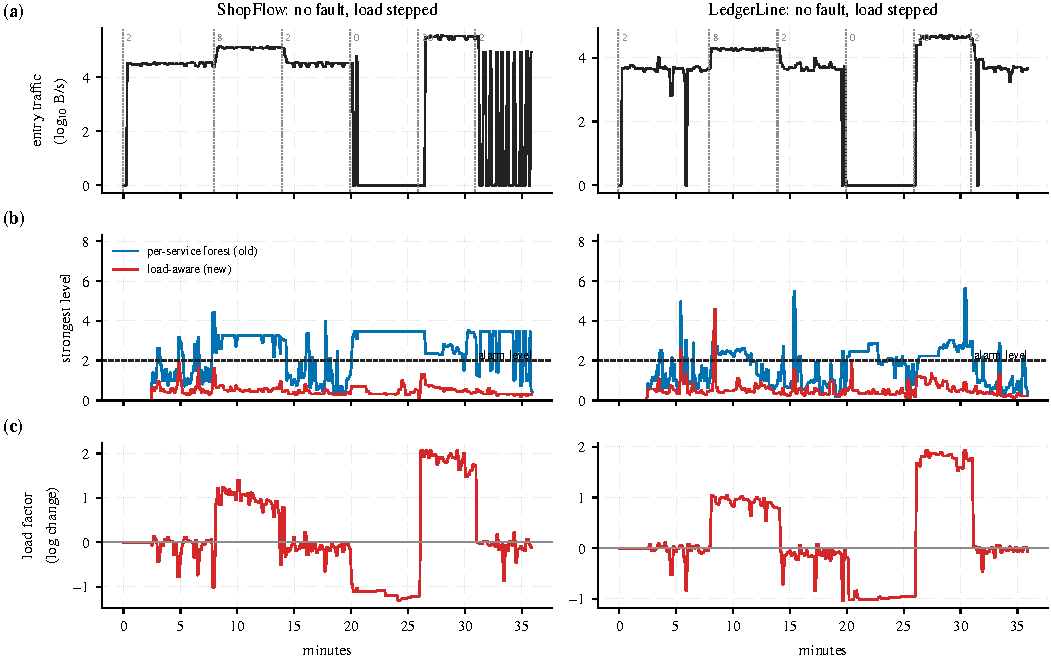
\includegraphics[width=0.98\textwidth]{fig_workload.pdf}
\caption{Two fault-free recordings with the load stepped (left ShopFlow, right LedgerLine). (a) Network traffic into the entry service. (b) The strongest service level of the old forest and of the load-aware model; the dashed line is the alarm level. (c) The load factor the new model read.}
\end{figure}

\begin{saybox}
``Panel (a) is the traffic going up and down. Panel (b) is the key: the old forest's level goes high every time the traffic changes, while the new model stays flat under the line. Panel (c) is why: the load factor follows the steps, so the model \emph{explains} the change instead of calling it a fault.''
\end{saybox}

\section{Hybrid: why have all three}
\begin{simplebox}
Rules react fast but fire on noise. ML is quiet and good at naming the source, but it needs warm-up and can absorb a slow fault. Container facts are the most reliable signal of all. The Hybrid alarms if \emph{any} of the three says so, and names the source using the ML ranking. We tuned one number: the rules alone only count if they go 25\% past their own line, so the Hybrid does not inherit all of the rule engine's false alarms.
\end{simplebox}
